\documentclass{scrbook}
\usepackage{graphicx} % Required for inserting images
\usepackage{tabularx} % Required for fixed width tables
\usepackage{scrlayer-scrpage} % Required for the subtitles
\usepackage{url} % Required for the URLs
\usepackage{hyperref} % Required for the URLs
\usepackage{listings} % Required for the code snippets
\usepackage{mathtools} % Required for the system of equations
\usepackage{amsmath,amssymb} % Required for some math symbols
\usepackage{enumitem} % Required for lettered lists

% Put the caption of the snippets at the bottom
\lstset{
    captionpos=b
}


\title{Blockchain and DLTs generalities}
\subtitle{Ambient intelligence course (A.Y. 2025/2026)\\Topic taught by Prof. Arnaldo Tomasino}
\author{Gabriele Colapinto}
\date{\today}

\begin{document}

\maketitle
\thispagestyle{empty}

{\Large\textbf{License}} \\
{Notes from Ambient intelligence (A.Y. 2025/2026) by Gabriele Colapinto. 
Course taught by professors Michele Ruta, Floriano Scioscia, Arnaldo Tomasino, Davide Loconte — 
Licensed under CC BY-NC 4.0.\\
\url{https://creativecommons.org/licenses/by-nc/4.0/}}

\vspace*{\fill}
\rule{\textwidth}{0.2pt}
\small{© 2025 Gabriele Colapinto \\
Released under the \href{https://creativecommons.org/licenses/by-nc/4.0/}{Creative Commons Attribution–NonCommercial 4.0 International License}}

\clearpage

\tableofcontents

\chapter{Defining Blockchain: A Distributed Digital Ledger}

A blockchain is a distributed database enabling trustless collaboration of Decentralized Autonomous Organizations (DAOs). \\

Blockchain technology represents a new paradigm for recording and sharing information. Initially gaining prominence as the technology underpinning cryptocurrencies like Bitcoin, its applications now extend far beyond the financial domain. At its core, a blockchain is a novel data structure and protocol suite that allows multiple, distrusting parties to maintain a shared, immutable history of events without the need for a central administrator. This capability to create trust in a trustless environment is what makes the technology so transformative. \\

In essence, a blockchain can be defined as a \textbf{distributed database} structured as a \textbf{public ledger}, which is composed of a chronologically ordered \textbf{chain of records}, or blocks. It is distributed because the data is not stored on a single central server but is replicated and maintained by a wide variety of nodes across a peer-to-peer network. It functions as a ledger because it records transactions—digital events such as the transfer of an asset—in a verifiable and permanent way. \\


The strategic departure from traditional data management systems is best understood by comparing a blockchain to a conventional database.

\begin{table}[h]
    \centering
    \begin{tabular}{|p{0.3\textwidth}|p{0.3\textwidth}|p{0.3\textwidth}|}
    \hline
    \textbf{Attribute} & \textbf{Traditional Database} & \textbf{Blockchain} \\
    \hline
    \textbf{Data Storage \& Control} & Centralized; data is stored and managed on a central node or by a single authority. & Decentralized; data is distributed and maintained by all participating nodes in the network. \\
    \hline
    \textbf{Data Mutability} & Data is mutable; a trusted administrator can alter, add, or delete records. & Data is immutable; once a transaction is recorded in a block, it can never be changed or erased. \\
    \hline
    \textbf{Trust Model} & Requires a trusted third party or mediator to validate transactions and safeguard records. & "Trustless"; trust is established by cryptographic principles and consensus protocols, not by an intermediary. \\
    \hline
    \end{tabular}
    \caption{Comparison between Traditional Database and Blockchain}
\end{table}

The genesis of modern blockchain can be traced to a 2008 whitepaper titled "Bitcoin: A Peer-to-Peer Electronic Cash System," published by an individual or group using the pseudonym Satoshi Nakamoto. The subsequent implementation of Bitcoin, released in January 2009, provided the first successful, large-scale demonstration of the technology. Before Bitcoin, research into Distributed Ledger Technologies (DLT) was not highly active, as the associated technical and organizational issues were largely seen as unsurmountable. However, Bitcoin's breakthrough was so significant because it proved that these problems could be solved. Consequently, both the \textbf{success and the limitations} of the Bitcoin platform provided the fuel for a new wave of research into DLT, aimed at improving and expanding upon the original concepts. \\

These unique properties are a direct result of its innovative architectural design, which combines cryptography, peer-to-peer networking, and distributed consensus.

\chapter{The Architecture of a Blockchain}

\begin{figure}[htbp]
    \centering
    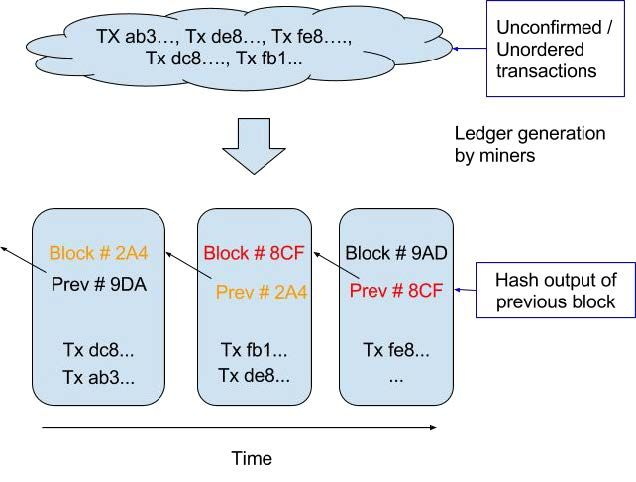
\includegraphics[width=\linewidth]{Images/Blockchain_architecture.jpg}
    \caption{Blockchain architecture -- The fact that each block has a link to the previous one means that the blockchain can be traversed backwards as a simply linked list.}
    \label{fig:blockchain_architecture}
\end{figure}

The security, immutability, and transparency of a blockchain are not abstract concepts; they are direct consequences of its unique data structure. This architecture is a convergence of several established computer science techniques, organized in a way that creates a system where data, once recorded, is exceptionally difficult to alter. Understanding this structure is fundamental to appreciating how a blockchain functions. \\


The blockchain architecture is composed of three primary components: transactions, blocks, and the chain itself.

\begin{enumerate}
    \item \textbf{Transactions:} A transaction is a record of a digital event. While initially used for financial transfers, a transaction can represent the transfer of any digital asset or the recording of any agreed-upon data. In a blockchain network, transactions are protected using asymmetric cryptography. Each participant, or peer, is identified by a public key and possesses a corresponding private key. To authorize a transaction, a peer signs it with their private key, creating a digital signature that can be verified by anyone else using the sender's public key.
    
    \item \textbf{Blocks:} A block is an ordered batch of transactions that have been cryptographically validated and are proposed to be added to the ledger. By grouping transactions into blocks, the blockchain processes updates to its state in discrete, chronologically linked intervals. This block serves as a batch update to the shared ledger. The number of blocks preceding a specific block in the chain is called \textbf{block height}. To remember this terminology we can think of the blockchain as a vertical structure growing upwards.
    
    \item \textbf{The Chain:} The chain is the crucial element that ensures the chronological and tamper-evident nature of the ledger. Each block is cryptographically linked to the one that came before it. This is achieved by including the cryptographic hash of the preceding block within the header of the current block. A hash is a unique, fixed-length string of characters generated from the block's contents. If even a single piece of data in a previous block were to be altered, its hash would change, which would in turn invalidate the hash in the subsequent block, and so on, creating a cascade effect that would be immediately detectable by the entire network. This linking mechanism makes the ledger indelible.
\end{enumerate}

The very first block in any blockchain is a special case known as the \textbf{Genesis Block}. It has a different structure because it has no preceding block to reference. It serves as the foundation upon which all subsequent blocks are built, with a block height of 0. \\

Understanding this static structure is the first step; the next is to explore the dynamic process by which new transactions are validated and permanently incorporated into this chain.

\chapter{The Lifecycle of a Transaction}

To appreciate how a blockchain operates, it is essential to understand the journey of a single transaction. This lifecycle details the process by which a proposed event, created by a single participant, becomes a permanent, globally verified record on the distributed ledger. This multi-step process ensures that only valid transactions are added to the chain in a consistent and agreed-upon order. \\


A transaction follows a clear, sequential path from its creation to its final inclusion in the blockchain:

\begin{enumerate}
    \item \textbf{Creation and Broadcast:} A peer initiates the process by creating a transaction, such as sending a digital asset to another peer. This transaction is signed with the originator's private key to prove ownership and authenticity. The signed transaction is then broadcast to all other nodes in the peer-to-peer network.
    
    \item \textbf{The Transaction Pool:} As nodes across the network receive broadcasted transactions, they do not immediately add them to the blockchain. Instead, they collect these signed but unconfirmed transactions in a temporary holding area. This data structure is commonly referred to as the \textbf{mempool} (in Bitcoin) or \textbf{txpool} (in some Ethereum implementations). Each node maintains its own transaction pool, which holds a set of pending transactions waiting to be included in a block. (See the cloud in figure ~\ref{fig:blockchain_architecture})
    
    \item \textbf{Block Proposal:} Periodically, nodes that participate in the block creation process (often called "miners") select a set of transactions from their transaction pool. They bundle these transactions into a new "candidate block," which they propose to the network as the next block to be added to the chain.
\end{enumerate}

With multiple nodes across the globe simultaneously selecting different sets of transactions to create their own candidate blocks, the network is immediately faced with multiple, competing versions of the next block. The fundamental challenge, therefore, is not just choosing a block, but resolving this inherent conflict to maintain a single history. This is the critical role of a consensus protocol.

\chapter{Achieving Agreement: Consensus Protocols}

\begin{figure}
    \centering
    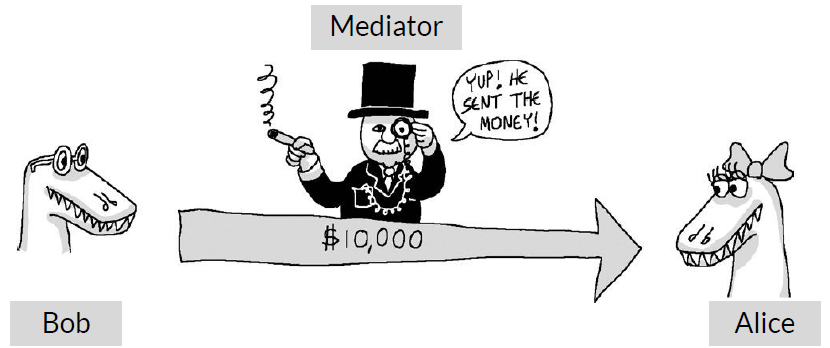
\includegraphics[width=0.5\linewidth]{Images/Transaction_with_central_authority.png}
    \caption{Transaction in a system with a central authority}
    \label{fig:transaction_central_authority}
\end{figure}

\begin{figure}
    \centering
    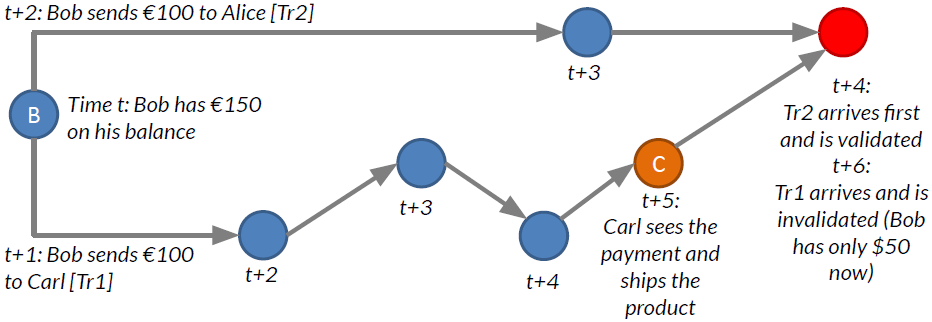
\includegraphics[width=\linewidth]{Images/Double_spending_problem.png}
    \caption{Double spending problem}
    \label{fig:double_spending_problem}
\end{figure}

\begin{figure}
    \centering
    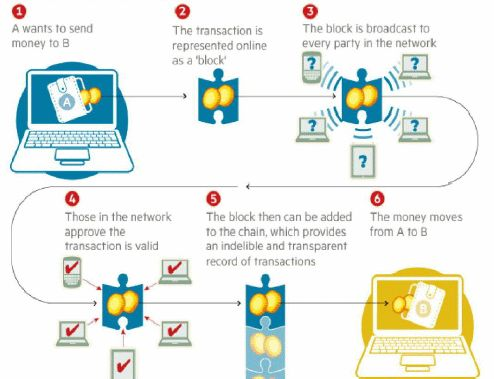
\includegraphics[width=0.7\linewidth]{Images/Blockchain_transaction.jpg}
    \caption{Blockchain transaction}
    \label{fig:blockchain_transaction}
\end{figure}

In any distributed system lacking a central authority, the primary challenge is achieving network-wide agreement. Blockchains require a formal consensus protocol to ensure every node maintains an identical copy of the ledger, thereby preventing fraud and guaranteeing the integrity of the record.

\section{The double spending problem}

A primary threat that consensus protocols are designed to prevent is the \textbf{"Double Spending"} problem (See figure ~\ref{fig:double_spending_problem}). In a digital system, it is trivial to copy data. This creates a vulnerability where a malicious actor could attempt to spend the same digital asset more than once. For example, Bob, with a balance of 150 €, could create two separate transactions: one sending 100 € to Alice and another sending 100 € to Carl. He could then broadcast both to the network. The vulnerability exists because Alice and Carl might act on the transaction \textit{before} the network has reached a global consensus. If they were to ship their products as soon as they received the broadcast, only for one of the transactions to be later invalidated, one of them would be left unpaid. \\

One might think that the solution to this problem is to cerate a locking transaction involving the issuer of the payment, the receiver of the payment and all the possible nodes in between them. In other words, let's say that Bob wants to send money to Alice. Bob communicates to Alice that he wants to send money and all the nodes involved in the transaction, including the possible nodes in the middle, are locked until the transaction is completed. Bob can't issue another payment and Alice can't receive another payment until the current payment is completed. That would be a possible solution based on a strategy used in other distributed systems but it would be \textbf{terribly suboptimal!} Bitcoin is designed to be more dynamic and to have a vast amount of users. Using this blocking strategy is feasible in a small network of users who issue a small number of transactions. We need to use a different strategy in a context with millions of users and millions of transactions. Let's say that an e-commerce website accepts Bitcoin as a form of payment. If we were to block the website for every payment it would mean that the website cannot receive simultaneous payments from different accounts and this would cause a denial of service to the great majority of the users at any given time. \\

The blockchain protocol solves the double spending problem using a different strategy. It creates a clear distinction between a broadcasted transaction (which is merely a proposal) and a confirmed transaction (which is an immutable record). A transaction is considered valid and final \textbf{only when it is included in a confirmed block} that is part of the accepted chain. (See figure ~\ref{fig:blockchain_transaction})\\

\section{Proof of Work (PoW)}

\begin{figure}[htbp]
    \centering
    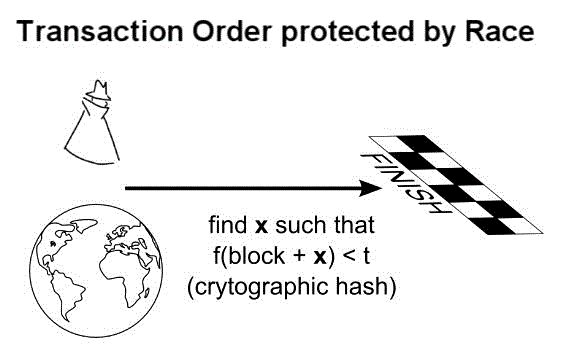
\includegraphics[width=0.7\linewidth]{Images/Proof_of_work.jpg}
    \caption{Proof of Work (PoW) -- In the figure 'x' is the nonce, the 'block' variable comprises both the transactions and the hash of the previous block and 't' is the threshold.}
    \label{fig:pow}
\end{figure}

\textbf{Proof of Work (PoW)} was the first and foundational consensus protocol, introduced by Bitcoin. It establishes a fair and verifiable method for choosing which node gets to add the next block to the chain. PoW frames this decision as a competitive "race" among nodes to solve a computationally difficult mathematical challenge. The first node to solve the challenge wins the right to have its block added to the chain. \\

The PoW challenge is designed to be difficult to solve but trivial for others to verify. The challenge requires finding a specific value known as a \textbf{nonce}.

\begin{itemize}
    \item A \textbf{nonce} is an arbitrary number that can be used just once. In the context of PoW, it is an input to the block's hashing function. Nodes must find a nonce value that, when combined and hashed with the block's transactions and the previous block's hash, produces a new hash that is below a specific target value, or threshold. (See figure ~\ref{fig:pow})
    
    \item \textbf{Mining} is the process whereby nodes, called miners, dedicate immense computational resources to repeatedly guess nonce values until they find one that satisfies the requirement. The first miner to find a valid nonce broadcasts their block and the solution to the network. Other nodes can quickly verify that the hash is correct, confirming the "proof of work" and accepting the new block. The difficulty of this challenge can be adjusted to ensure a consistent block creation rate. For instance, the Bitcoin network adjusts the hash threshold every 2016 blocks to maintain an average block time of 10 minutes. For their effort, miners are rewarded, typically with newly created units of the blockchain's native currency.
\end{itemize}

\section{Specialized Hardware: ASICs}

The computational expense of mining has grown exponentially on major PoW blockchains. While miners initially used standard CPUs and later more powerful GPUs, the process is now dominated by specialized hardware.

\begin{itemize}
    \item An \textbf{Application-Specific Integrated Circuit (ASIC)} is an integrated circuit chip customized for a particular use. Miners now use ASICs that are designed for the single purpose of performing the hashing calculations required for PoW. These devices are orders of magnitude more efficient than general-purpose hardware, making them essential for competitive mining.
\end{itemize}

The high energy and resource consumption of PoW has been a significant drawback, leading to the development of numerous alternative consensus protocols, such as Proof of Stake (PoS), that aim to achieve consensus with greater efficiency. \\

While PoW provides a mechanism for selecting the next block, the distributed nature of the network can lead to situations where multiple miners solve the challenge almost simultaneously, creating a temporary disagreement about the state of the chain.

\chapter{Maintaining Chain Integrity: Forks and Finality}

A blockchain's value is contingent on its status as a single, canonical source of truth. Therefore, its protocol must possess an automated and deterministic mechanism for resolving the inevitable conflicts that arise in a distributed environment, ensuring the network always converges on one history. \\

This situation leads to a \textbf{"fork"} in the blockchain. A fork occurs when two or more miners solve the PoW challenge at approximately the same time and broadcast their respective valid blocks to the network. Due to network latency, some nodes will receive one block first, while other nodes will receive the other. This results in two competing, valid versions of the blockchain existing simultaneously on different parts of the network. \\


To resolve this ambiguity, blockchain protocols like Bitcoin's implement a simple yet powerful resolution mechanism: the \textbf{"longest chain rule."} \\

The rule dictates that nodes will always consider the chain with the greatest number of blocks to be the valid one. This rule is not arbitrary; it is a fundamental principle of Proof of Work. The longest chain is, by definition, the one that has had the most computational work and energy expended on it, and therefore represents the consensus of the majority of the network's hashing power. As new blocks are mined, one chain will inevitably grow longer than the other. When a node receives information that a competing chain has become longer than the one it was working on, it will abandon its current chain and switch to the longest one. The blocks on the shorter, discarded chain are abandoned, and their transactions are returned to the transaction pool to be included in a future block. \\

This mechanism directly relates to the concept of \textbf{transactional finality}. A transaction included in a block is not considered fully secure immediately. However, its security increases with every subsequent block added to the chain on top of it. The deeper a block is buried in the chain, the more computationally difficult it becomes to alter it, because an attacker would have to re-mine not only that block but all the blocks that follow it, and do so faster than the rest of the network. For Bitcoin, it is considered practically unfeasible to revert a transaction that is six or more blocks deep in the chain. (See figure ~\ref{fig:growing_the_blockchain})\\

Through mechanisms like the longest chain rule, the blockchain ensures that despite temporary forks, the network will always converge toward a single, immutable history, which is the foundation of its integrity and reliability.

\begin{figure}
    \centering
    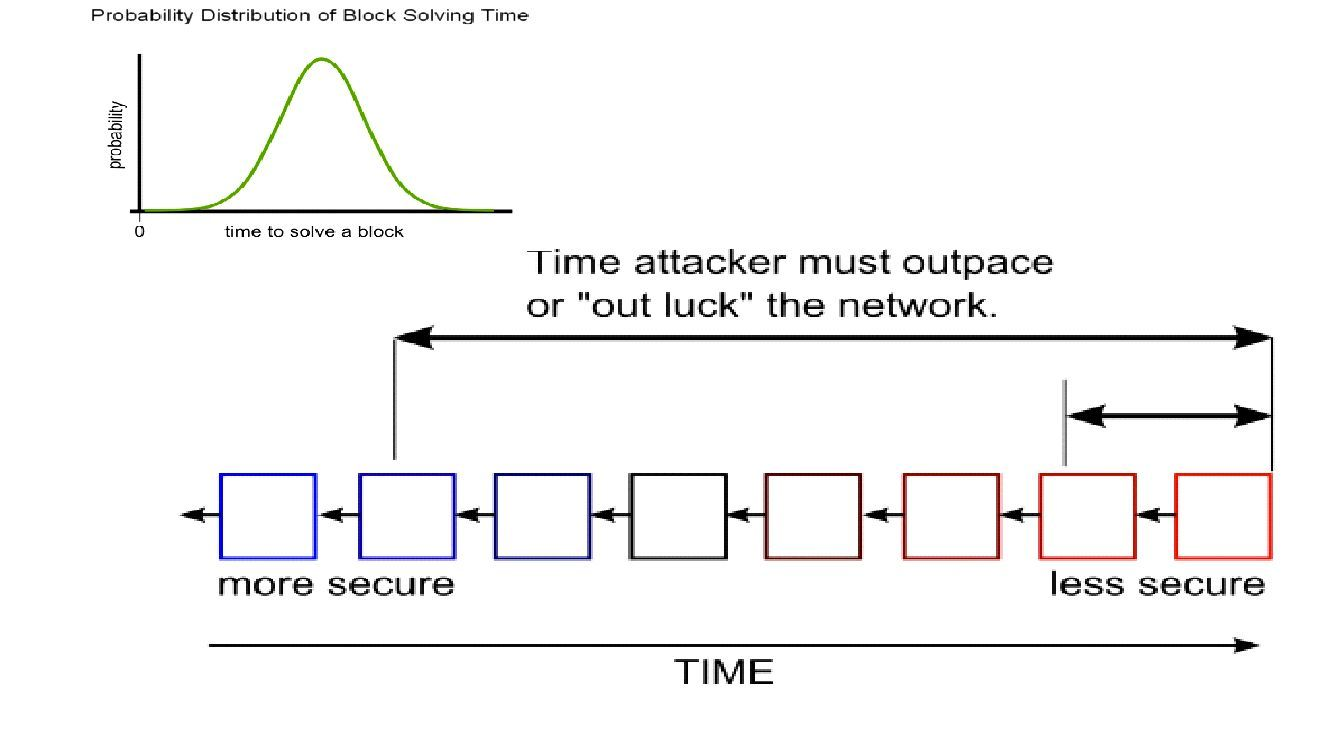
\includegraphics[width=\linewidth]{Images/Growing_the_blockchain.jpg}
    \caption{As the blockchain grows the old blocks become more secure.}
    \label{fig:growing_the_blockchain}
\end{figure}

\chapter{Summary of Key Blockchain Properties}

The architecture, transaction lifecycle, and consensus mechanisms previously discussed give rise to a unique set of properties that define blockchain technology. These characteristics, when combined, create a powerful framework for building decentralized applications and systems where security and integrity are embedded into the protocol itself, rather than being managed by a central intermediary. \\

The core properties that emerge from a blockchain's design include:

\begin{itemize}
    \item \textbf{Robustness and Integrity:} The system is designed as a distributed peer-to-peer network that is tolerant to individual node failures. The integrity of every transaction is guaranteed by the consensus protocol, which ensures all nodes agree on a single history.
    
    \item \textbf{Authentication and Non-Repudiation:} The use of digital signatures derived from asymmetric cryptography ensures that the originator of a transaction is verifiable and cannot later deny their authorization (non-repudiation).
    
    \item \textbf{Transparency and Verifiability:} Because all confirmed transactions are recorded on the shared public ledger, the history of any digital asset is transparent and can be independently audited by any participant in the network.
    
    \item \textbf{Decentralization:} The network operates without a central authority or trusted third party. It enables collaboration and interaction among participants who do not need to explicitly trust one another, as trust is placed in the protocol itself.
    
    \item \textbf{Tamper-Proof Nature:} The combination of cryptographic hashing and distributed consensus makes the ledger extraordinarily difficult to alter. No single node or small group of colluding nodes can force the addition, removal, or modification of data. The term "small" is specifically characterized as a maximum percentage of all participating nodes; the actual value of this threshold depends on the particular consensus mechanism being used. In the specific case of the Bitcoin, the Proof of Work consensus mechanism makes the system \textbf{Byzantine Fault Tolerant (BFT)} making the maximum amount of malicious nodes equal to one third of all the nodes in the network.
    
    \item \textbf{Pseudonymity:} Users on the blockchain are not identified by their real-world identities but by their cryptographic keys (e.g., their public key or address). The system sees a user as a set of cryptographic material, not as a specific person or organization.
\end{itemize}

It is crucial to understand the distinction between \textbf{pseudonymity and anonymity}. While a user's real-world identity is not directly linked to their blockchain address, the system is not truly anonymous. All transactions are public and traceable on the ledger. By analyzing transaction patterns, it is possible to reconstruct activity and, in some cases, link a pseudonymous identity to a real-world entity. This technique is used in data analysis, law enforcement, and counter-terrorism efforts. \\

Collectively, these properties create a powerful framework for building systems where security, transparency, and integrity are programmatically guaranteed, heralding new possibilities for digital interaction and exchange.

\chapter{Applications of Blockchain and DLTs}

While blockchain technology's initial success was inextricably linked to cryptocurrencies like Bitcoin, its fundamental strengths—immutability, traceability, and trustless verification—have established it as a general-purpose technology. Its potential extends far beyond financial services, with innovative applications emerging in a wide range of both financial and non-financial sectors, transforming traditional processes and creating new opportunities for efficiency and transparency.

\section{Smart contracts}

First defined by Nick Szabo in 1994, a smart contract is "a computerized transaction protocol that executes the terms of a contract". In the context of a blockchain, a smart contract is a piece of code registered on the ledger as an asset itself. This code is collectively verified and validated by all network participants, effectively creating an immutable contract that automatically executes its terms when predefined conditions are met. \\

Smart contracts can be implemented using a variety of formalisms, providing flexibility for developers across different platforms.

\begin{itemize}
    \item \textbf{General-Purpose Programming Languages:} Pre-existing languages such as \texttt{Java} or \texttt{Python} are used for platforms like Hyperledger Fabric.
    
    \item \textbf{Purpose-Built Languages:} To facilitate the creation of smart contracts on specific platforms, specialized languages were developed, most notably \texttt{Solidity} for the Ethereum platform.
    
    \item \textbf{Logical Languages and Automata:} Other formalisms, including logical languages and automata, can also be used to define the rules and execution flow of smart contracts.
\end{itemize}

By codifying contractual obligations into an immutable and self-executing format, blockchain and smart contracts provide a powerful framework for automating and securing transactions across a multitude of industries.

\section{Insurance}

Assets such as vehicles, which can be uniquely identified by a Vehicle Identification Number (VIN), can be registered on a blockchain. This process creates an immutable and traceable history of all significant events related to the asset, including changes of ownership and accidents. Any insurance company can then access and verify this history to assess risk and process claims, thereby minimizing reliance on trusted intermediaries, reducing informational asymmetries, and creating a verifiable audit trail that mitigates fraudulent claims.

\section{Notary Services}

Registering a document on a blockchain provides legally binding \textbf{Proof of Existence}, confirming the document existed at a specific time; \textbf{Proof of Ownership}, linking it to a particular identity; and \textbf{Proof of Integrity}, ensuring it has not been tampered with. This capability eliminates the need for traditional notarization services and their associated fees, making document verification more efficient and accessible.
    
\section{Digital Content Markets}

In industries like music, determining royalty payments has historically been a convoluted process. Blockchain offers a solution by maintaining a comprehensive and accurate distributed database of music rights ownership. Smart contracts can be programmed to automatically calculate and distribute royalty splits to all stakeholders whenever a song is streamed or sold. Initiatives like \texttt{Soundreef} and \texttt{JAAK} have pioneered this approach to bring transparency and automation to royalty management.
    
\section{Decentralized Storage}

In contrast to traditional cloud storage solutions like Dropbox or Google Drive where users must trust a third-party service provider with their data, blockchain-based storage offers a decentralized alternative. In this model, files are split into pieces and distributed across a peer-to-peer network of nodes. Users can not only store their own data securely but also participate in the network by sharing their own unused bandwidth and disk space in return for cryptocurrency payments.
    
\section{Internet of Things (IoT)}

The conventional centralized model for IoT, where a central hub controls all interactions between devices, is impractical for scenarios requiring autonomous machine-to-machine communication. Blockchain provides a decentralized platform for secure and trusted data exchange between devices. It serves as a general ledger, keeping an immutable record of all messages and transactions exchanged within an IoT topology. To address the challenges of resource-constrained IoT environments, evolutions like \texttt{IOTA} have been developed, which use a Directed Acyclic Graph (DAG) data structure instead of a traditional chain to enable scalable and feeless data marketplaces for devices.
    
\section{Anti-Counterfeit Solutions}

The immutable and traceable characteristics of blockchain are exceptionally well-suited for supply chain management and anti-counterfeit solutions. By storing a product's details and journey as a series of transactions on a blockchain, its authenticity can be verified at any point from production to sale. This application is gaining significant traction, particularly in the agri-food sector, where proof of origin and authenticity is paramount. \\

The breadth of these applications underscores the versatility of distributed ledger technology, which is made possible by its sophisticated underlying data structures.

\end{document}
